\documentclass[12pt,ngerman]{beamer}


\usepackage[utf8]{inputenc}
\usepackage[T1]{fontenc}
\usepackage{booktabs}
\usepackage{babel}
\usepackage{graphicx}
\usepackage{csquotes}
\usepackage{xcolor}



\usepackage[]{listings}

%%%%%%%
\definecolor{hellgelb}{rgb}{1,1,0.8}
\definecolor{lightgelb}{rgb}{1,1,0.8}
\definecolor{colKeys}{rgb}{0,0,1}
\definecolor{colIdentifier}{rgb}{0,0,0}
\definecolor{colComments}{rgb}{1,0,0}
\definecolor{colString}{rgb}{0,0.5,0}


\lstset{%
		language={[LaTeX]TeX},%
		morekeywords={opening, closing, ifkomavarempty, ifkomavar,setkomavar, usekomavar},%
    float=hbp,%
    basicstyle=\ttfamily,%\footnotesize, %
    identifierstyle=\color{colIdentifier}, %
    keywordstyle=\color{colKeys}, %
    stringstyle=\color{colString}, %
    commentstyle=\color{colComments}, %
    literate={fl}{{f{}l}}2,%
    columns=flexible, %
    tabsize=2, %
    frame=single, %
    upquote=true,%
    extendedchars=true, %
    showspaces=false, %
    showstringspaces=false, %
    numbers=left, %
    numberstyle=\tiny, %
    breaklines=true, %
    backgroundcolor=\color{hellgelb}, %
    breakautoindent=true, %
    captionpos=b%
}




%%%%%%%%%%%%
\lstset{literate=%
    {Ö}{{\"O}}1
    {Ä}{{\"A}}1
    {Ü}{{\"U}}1
    {ß}{{\ss}}1
    {ü}{{\"u}}1
    {ä}{{\"a}}1
    {ö}{{\"o}}1
    {~}{{\textasciitilde}}1
}


\author{Uwe Ziegenhagen}
\title{Briefvorlagen mit \texttt{scrlttr2}}

\begin{document}


\begin{frame}

\maketitle

\end{frame}

\begin{frame}
\frametitle{Einführung}

\begin{itemize}
\item \enquote{ Ich finde, dass man Latex-Dokumenten meistens ansieht, dass sie in Latex gesetzt wurden, das stört mich, wenn ich auch die Vorteile erkenne.} und der Verweis auf \texttt{dinbrief}
\item \LaTeX-Layout muss nicht (schlecht) sein!
\item Für Briefe nutze ich \texttt{scrlttr2}, sehr flexibles Paket für Briefe, Teil von KOMA-Script
\item erlaubt (leichte) Anpassung an Design-Vorgaben
\item Ziel des Vortrags

\begin{itemize}
	\item Kurze Einführung in \texttt{scrlttr2}
	\item Erstellung von Briefvorlagen
\end{itemize}


\end{itemize}
\end{frame}

\begin{frame}
\frametitle{Klasse oder Umgebung}

\begin{itemize}
\item Traditionell: \texttt{scrlttr2} Dokumentenklasse
\item Seit einiger Zeit: \texttt{scrletter} Paket
\item MK empfiehlt Nutzung des Pakets
\item Im weiteren Vortrag Nutzung der Klasse mit \texttt{pdflatex}
\end{itemize}
\end{frame}


\begin{frame}[fragile]
\frametitle{Ein minimaler Brief}

\lstinputlisting[basicstyle=\ttfamily\footnotesize]{brief-01.tex}

\end{frame}

\begin{frame}[plain]
\frametitle{Ergebnis}

\begin{center}
\fbox{
\includegraphics[trim=0cm 14cm 0cm 3cm, width=1\textwidth]{brief-01}}
\end{center}
\end{frame}


\begin{frame}
\frametitle{Vordefinierte Variablen}

\texttt{scrlttr2} kennt eine Vielzahl vordefinierter Variablen, die sich befüllen lassen. Hier die wichtigsten: \vspace*{1em}

\begin{columns}
\begin{column}{0.3\textwidth}
\begin{itemize}
	\item backaddress
	\item customer
	\item date
	\item firstfoot
	\item firsthead
	\item fromaddress
	\item frombank
	\item fromemail
	\end{itemize}
\end{column}
\begin{column}{0.3\textwidth}
\begin{itemize}
	\item fromname
	\item fromfax
	\item fromphone
	\item fromurl
	\item invoice
	\item location
	\item myref
	\item nextfoot
	\end{itemize}
\end{column}
\begin{column}{0.3\textwidth}
\begin{itemize}
	\item nexthead
	\item place
	\item signature
	\item subject
	\item toname
	\item toaddress
	\item yourmail
	\item yourref
	\end{itemize}
\end{column}

\end{columns}

\end{frame}

\begin{frame}[containsverbatim]
\frametitle{Setzen und Nutzen von Variablen}

\textbf{Setzen von Variablen}

\begin{itemize}
	\item \lstinline|\setkomavar{Variable}{Wert}| weist der Variablen einen Wert zu
	\item \lstinline|\setkomavar{Variable}[Label]{Wert}| weist der Variablen einen Wert zu und setzt das Label
	\item \lstinline|\setkomavar*{Variable}{Label}| ändert nur das Label
\end{itemize}

\textbf{Nutzen von Variablen}

\begin{itemize}
	\item \lstinline|\usekomavar{Variable}| gibt Wert der Variablen zurück
	\item \lstinline|\usekomavar*{Variable}| gibt das Label zurück
\end{itemize}

\textbf{Nutzen von Variablen}

\begin{itemize}
	\item \lstinline|\ifkomavar{Variable}{dann}{sonst}| Fallunterscheidung
	\item \lstinline|\ifkomavarempty{Variable}{dann}{sonst}|  Fallunterscheidung
\end{itemize}


\end{frame}

\begin{frame}[fragile]
\frametitle{Setzen des Absenders}

\lstinputlisting[basicstyle=\ttfamily\footnotesize]{brief-02.tex}

\end{frame}

\begin{frame}[plain]
\frametitle{Ergebnis}

\begin{center}
\fbox{
\includegraphics[trim=0cm 15cm 0cm 0cm, width=1\textwidth]{brief-02}}
\end{center}
\end{frame}

\begin{frame}[fragile]
\frametitle{Setzen des Absenders}

\lstinputlisting[basicstyle=\ttfamily\footnotesize]{brief-03.tex}

\end{frame}

\begin{frame}[plain]
\frametitle{Ergebnis}

\begin{center}
\fbox{
\includegraphics[trim=0cm 15cm 0cm 0cm, width=1\textwidth]{brief-03}}
\end{center}
\end{frame}

\begin{frame}[fragile]
\frametitle{Anpassen der Variablen-Labels}

\lstinputlisting[basicstyle=\ttfamily\footnotesize]{brief-04.tex}

\end{frame}

\begin{frame}[plain]
\frametitle{Ergebnis}

\begin{center}
\fbox{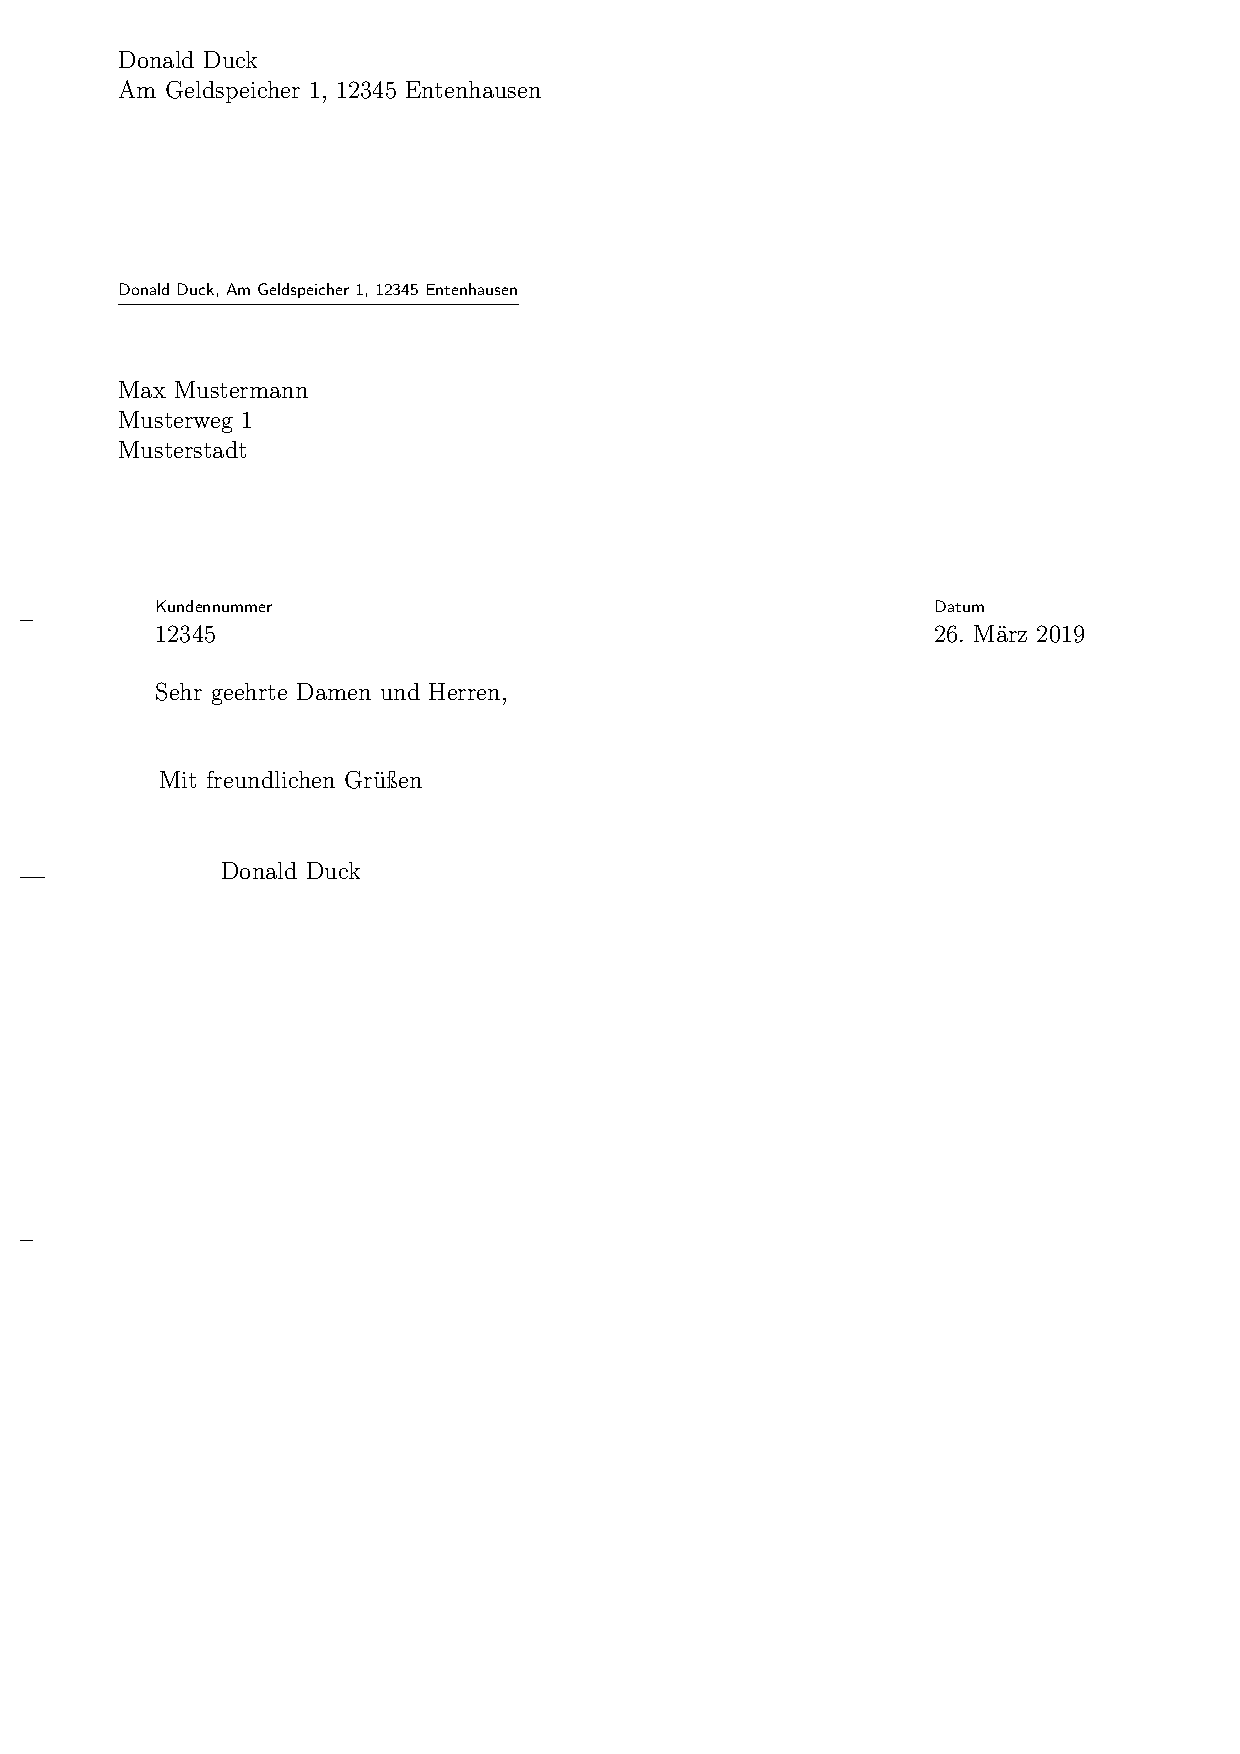
\includegraphics[trim=0cm 15cm 0cm 0cm, width=1\textwidth]{brief-04}}
\end{center}
\end{frame}

\begin{frame}[fragile]
\frametitle{Anpassen der Variablen-Labels}

\lstinputlisting[basicstyle=\ttfamily\footnotesize]{brief-05.tex}

\end{frame}

\begin{frame}[plain]
\frametitle{Ergebnis}

\vspace*{-0.35cm}\begin{center}
\fbox{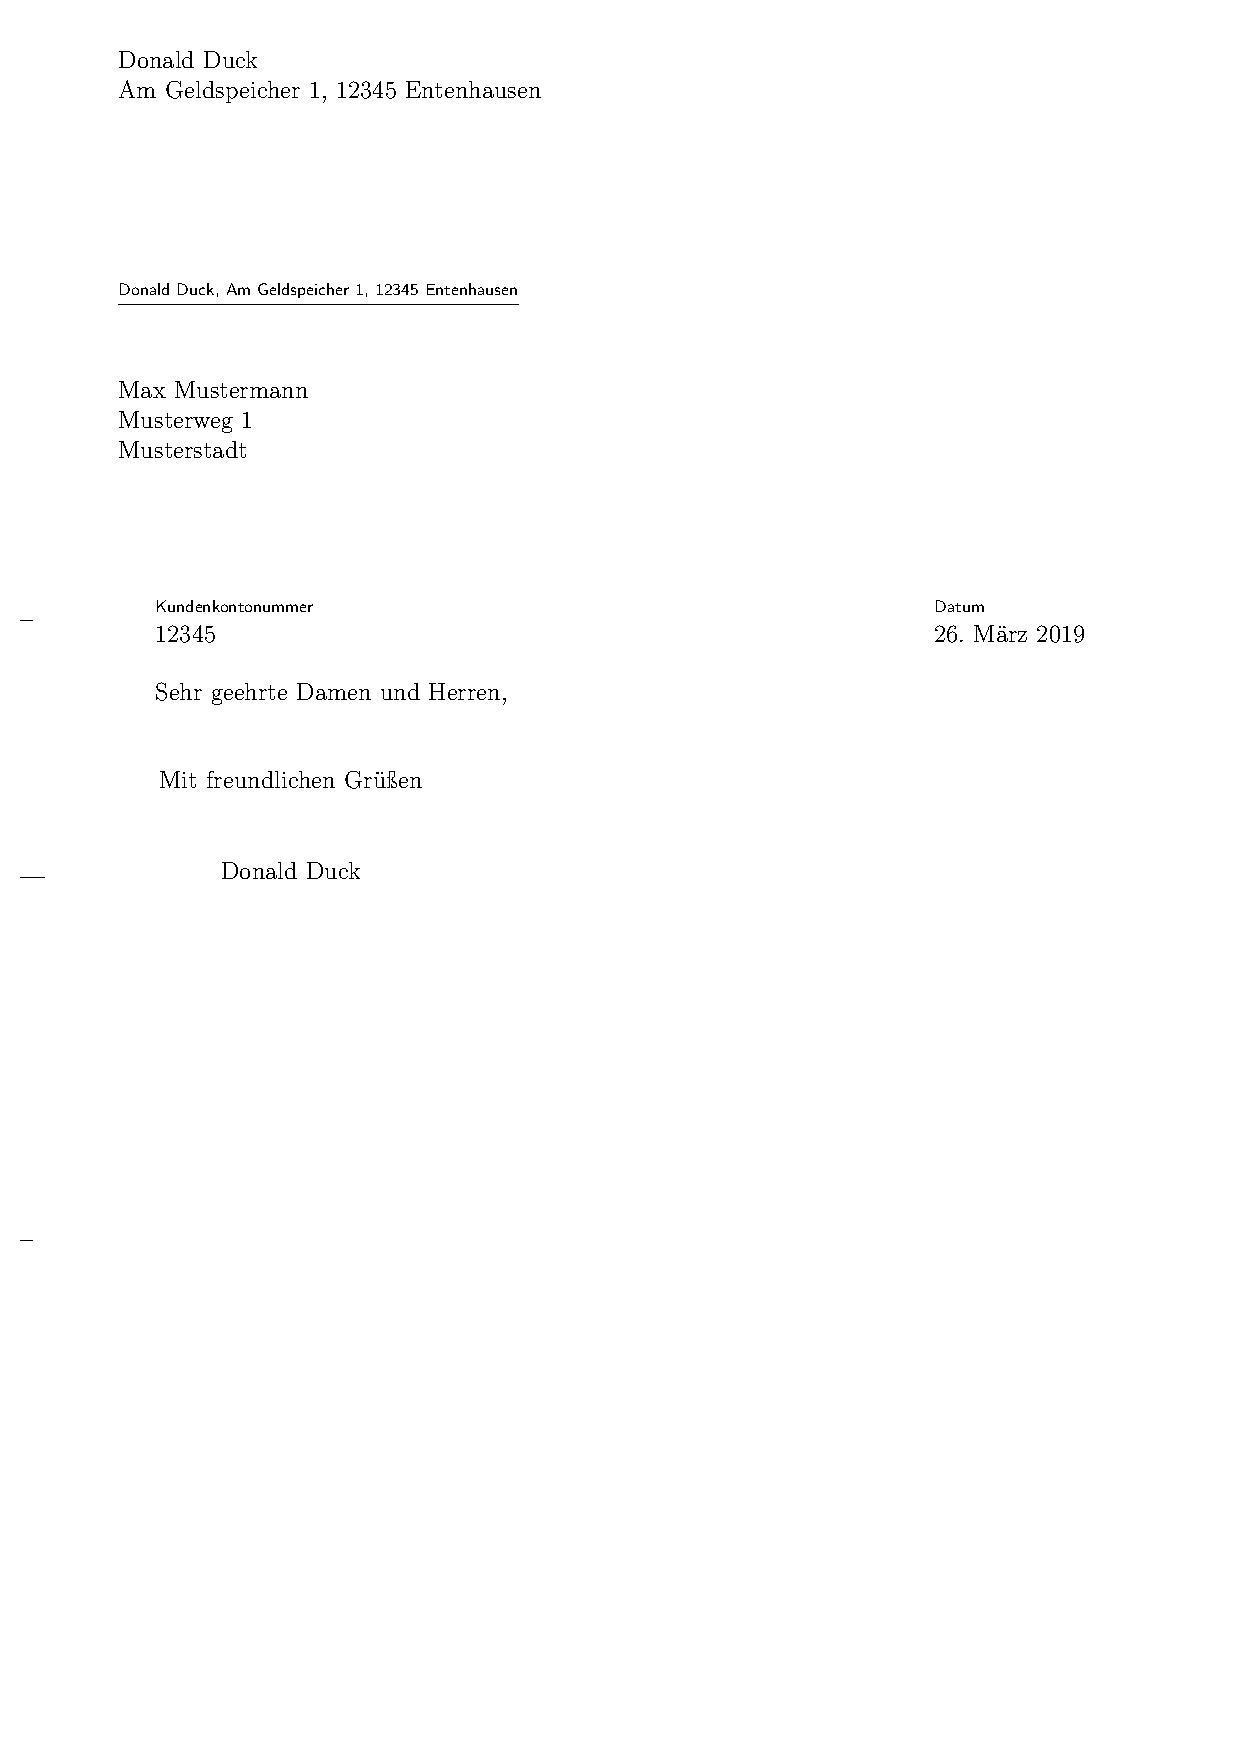
\includegraphics[trim=1cm 14.5cm 0cm 0.5cm, width=1\textwidth]{brief-05}}
\end{center}
\end{frame}


\begin{frame}[fragile]
\frametitle{Anpassen der Variablen-Labels}

\begin{itemize}
	\item Weitere wichtige Variablen

\begin{description}
\item[yourref] Fremde Briefreferenz 
\item[yourmail] Fremdes Briefdatum
\item[subject] Betreff
\item[title] Titel
\end{description}

\end{itemize}

\lstinputlisting[basicstyle=\ttfamily\footnotesize, firstline=5,lastline=13]{brief-06.tex}

\end{frame}

\begin{frame}[plain]
\frametitle{Ergebnis}

\vspace*{-0.75cm}\begin{center}
\fbox{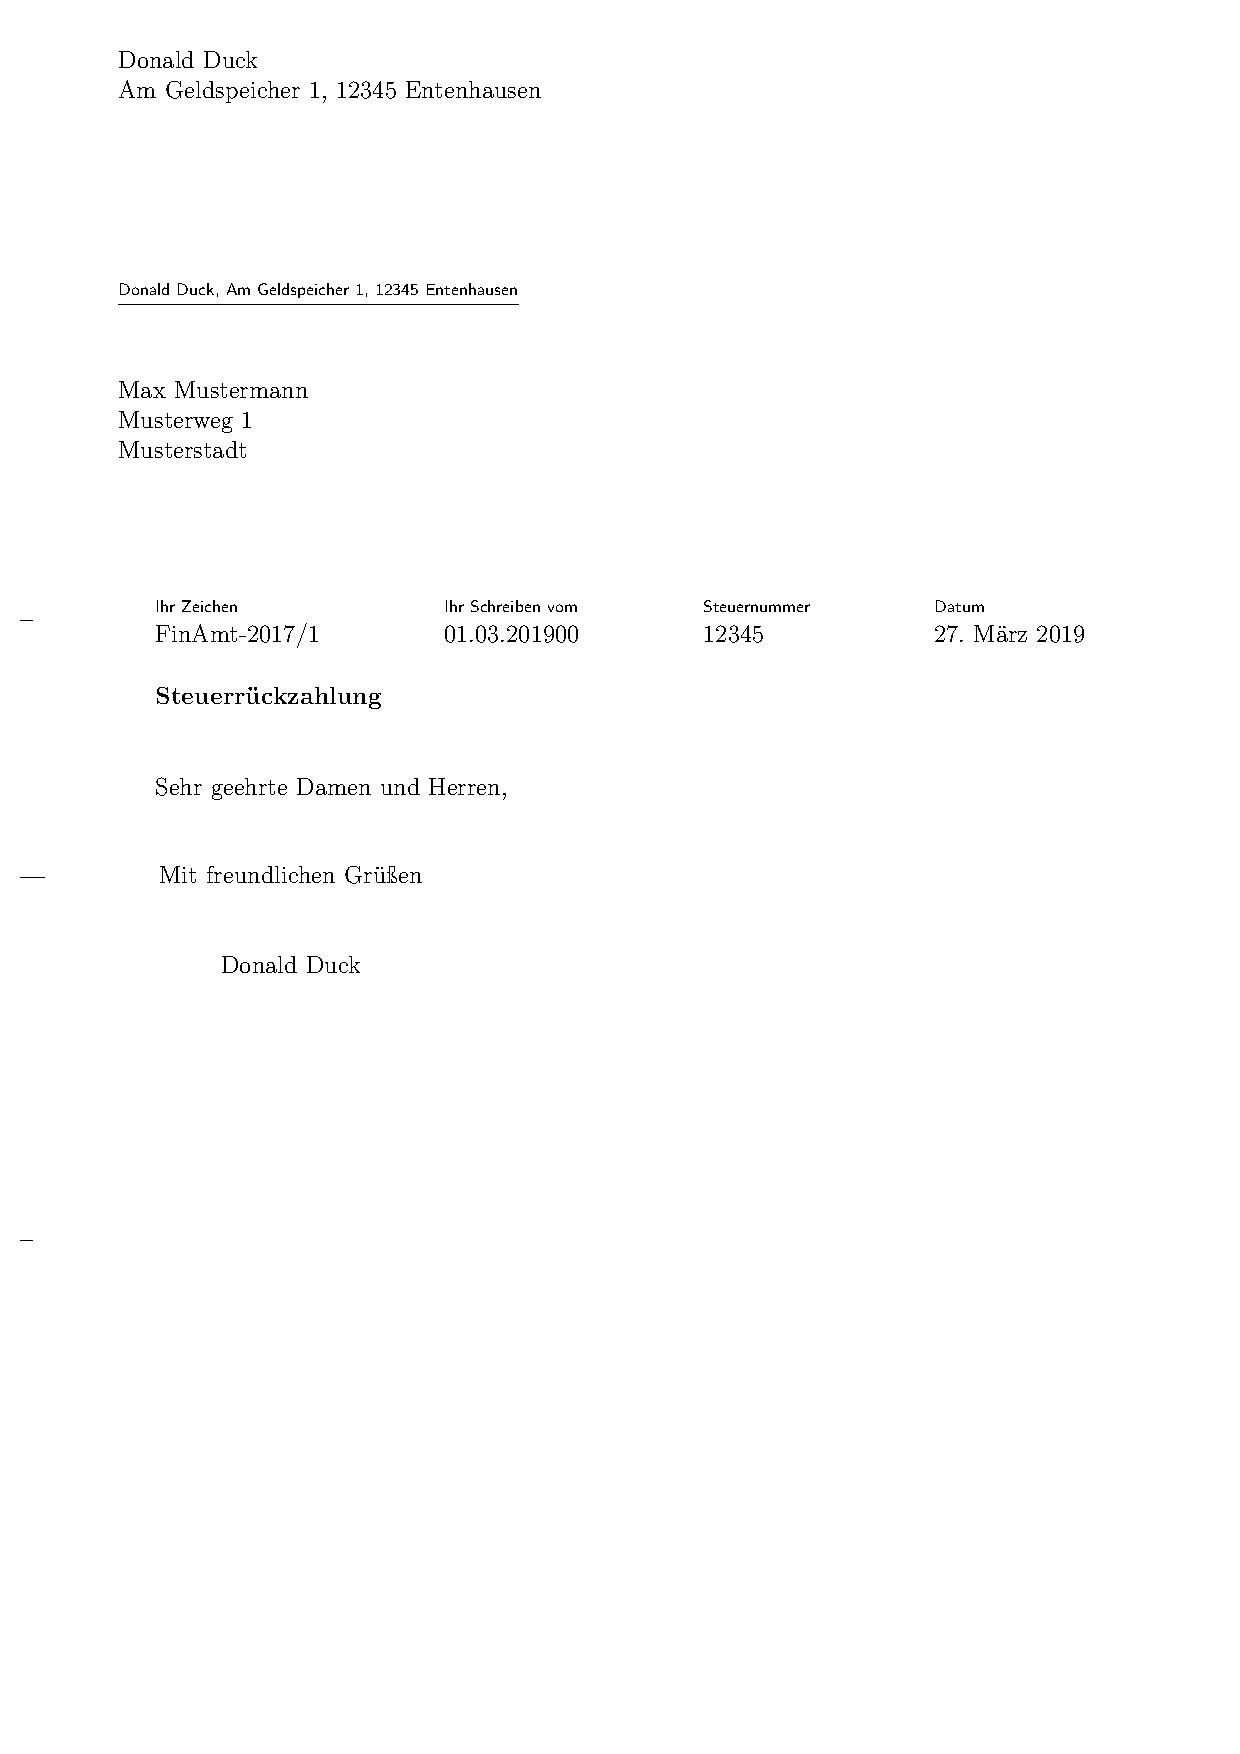
\includegraphics[trim=0cm 13.25cm 0cm 0.5cm, width=0.85\textwidth]{brief-06}}
\end{center}
\end{frame}


\begin{frame}[plain]
\frametitle{Übersicht aus der KOMA-Script Dokumentation}

\begin{center}
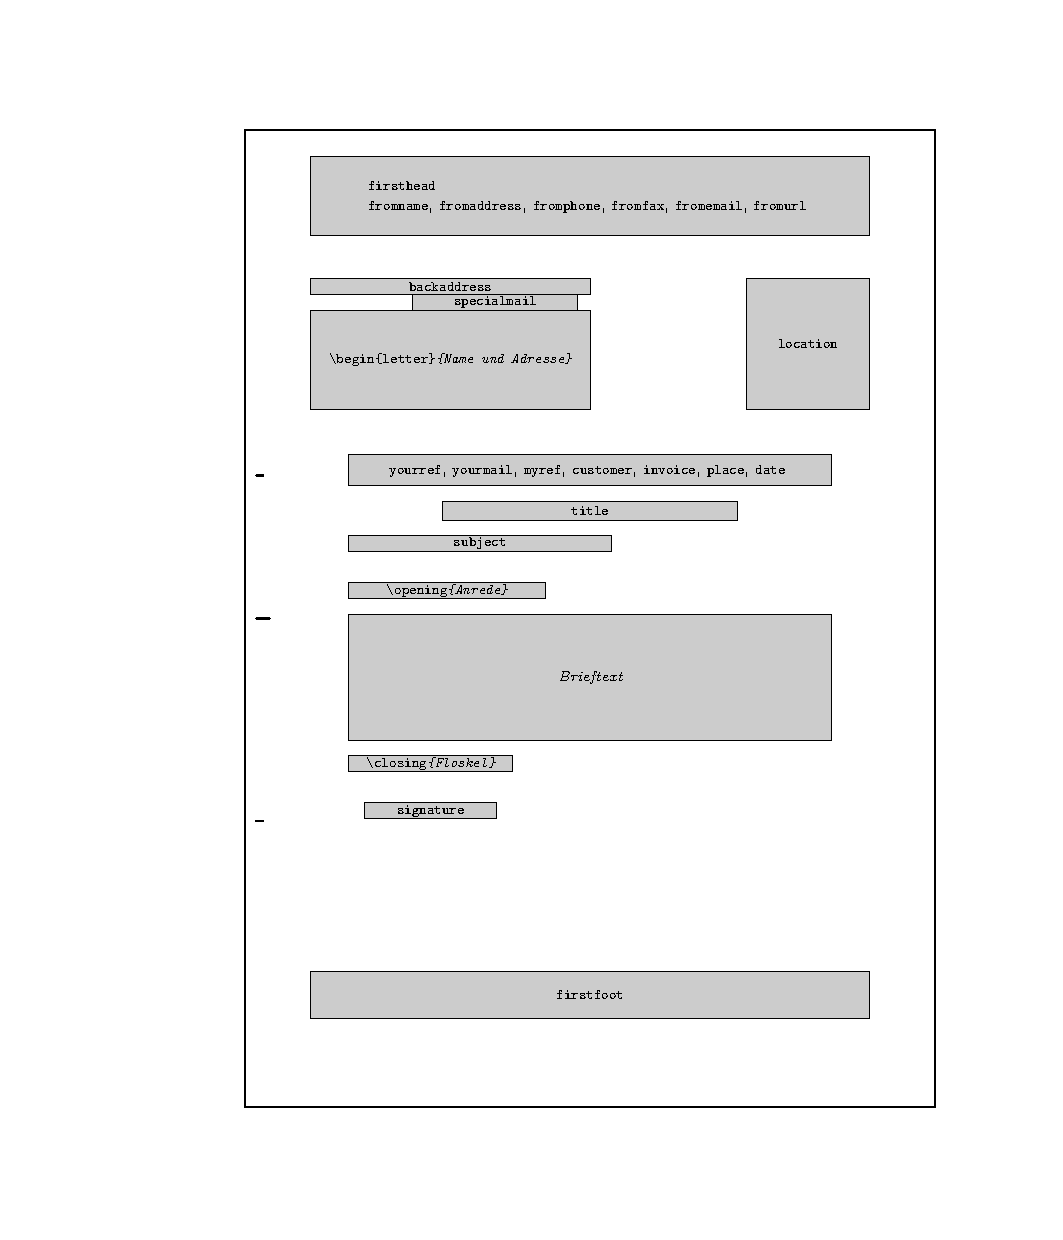
\includegraphics[width=0.5\textwidth]{scrguide193}
\end{center}
\end{frame}

\begin{frame}[containsverbatim]
\frametitle{Anpassungen des Layouts}

\begin{itemize}
\item \texttt{scrlttr2} bietet bereits interne Möglichkeiten zur Design-Anpassung
\begin{itemize}
	\item \texttt{fromalign} Ausrichtung der Absender-Anschrift, Standard ist \enquote{left}, mögliche Werte \enquote{center}, \enquote{right}, \enquote{off}
	\item Schriftart global, ganz global oder pro Element
	\item \enquote{geheime} Option: \texttt{egregdoesnotlikesansseriftitles} ändert Schriftart komplett auf Serifen-Schrift
	\end{itemize}
\end{itemize}
\end{frame}

\begin{frame}
\frametitle{fromalign=center}

\vspace*{-0.75cm}\begin{center}
\fbox{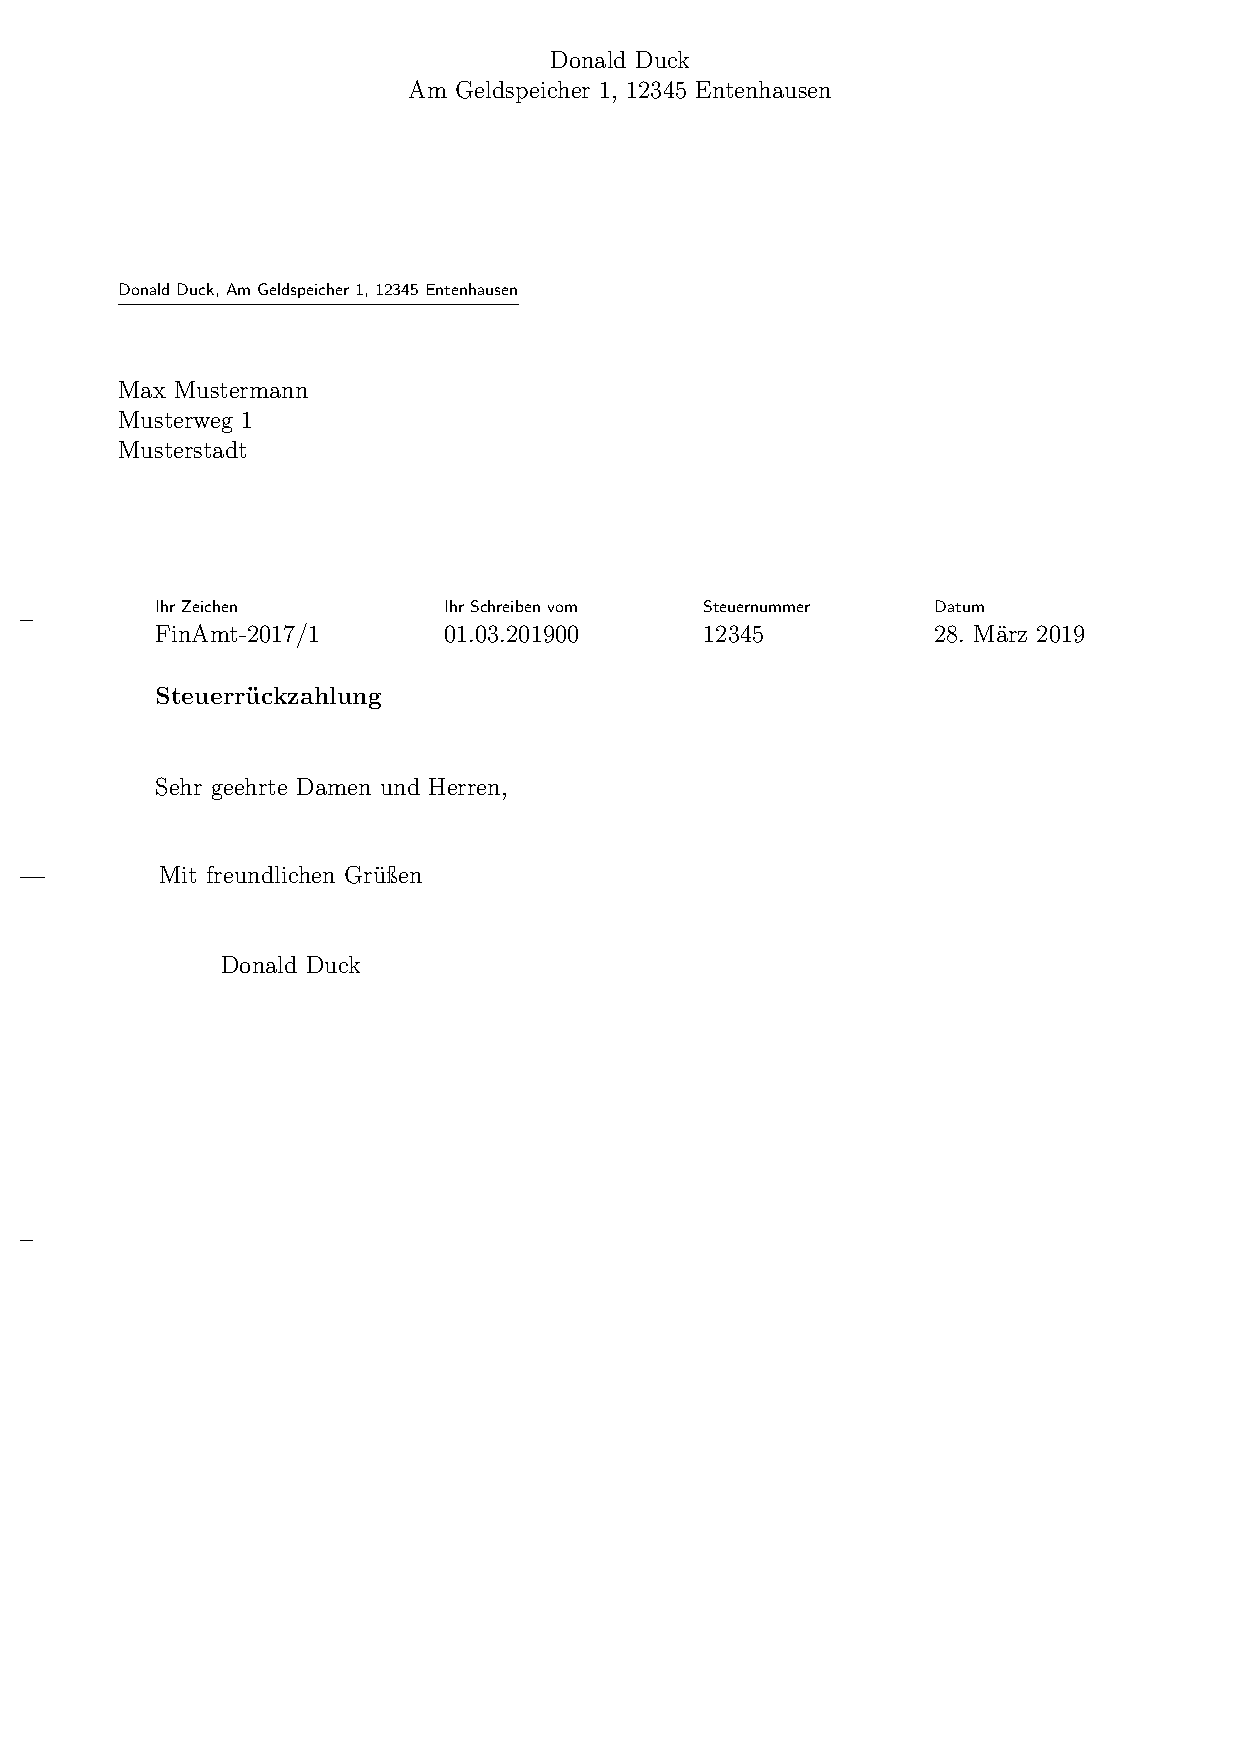
\includegraphics[trim=0cm 13.25cm 0cm 0.5cm, width=0.85\textwidth]{brief-07}}
\end{center}

\end{frame}


\begin{frame}
\frametitle{fromalign=right}

\vspace*{-0.75cm}\begin{center}
\fbox{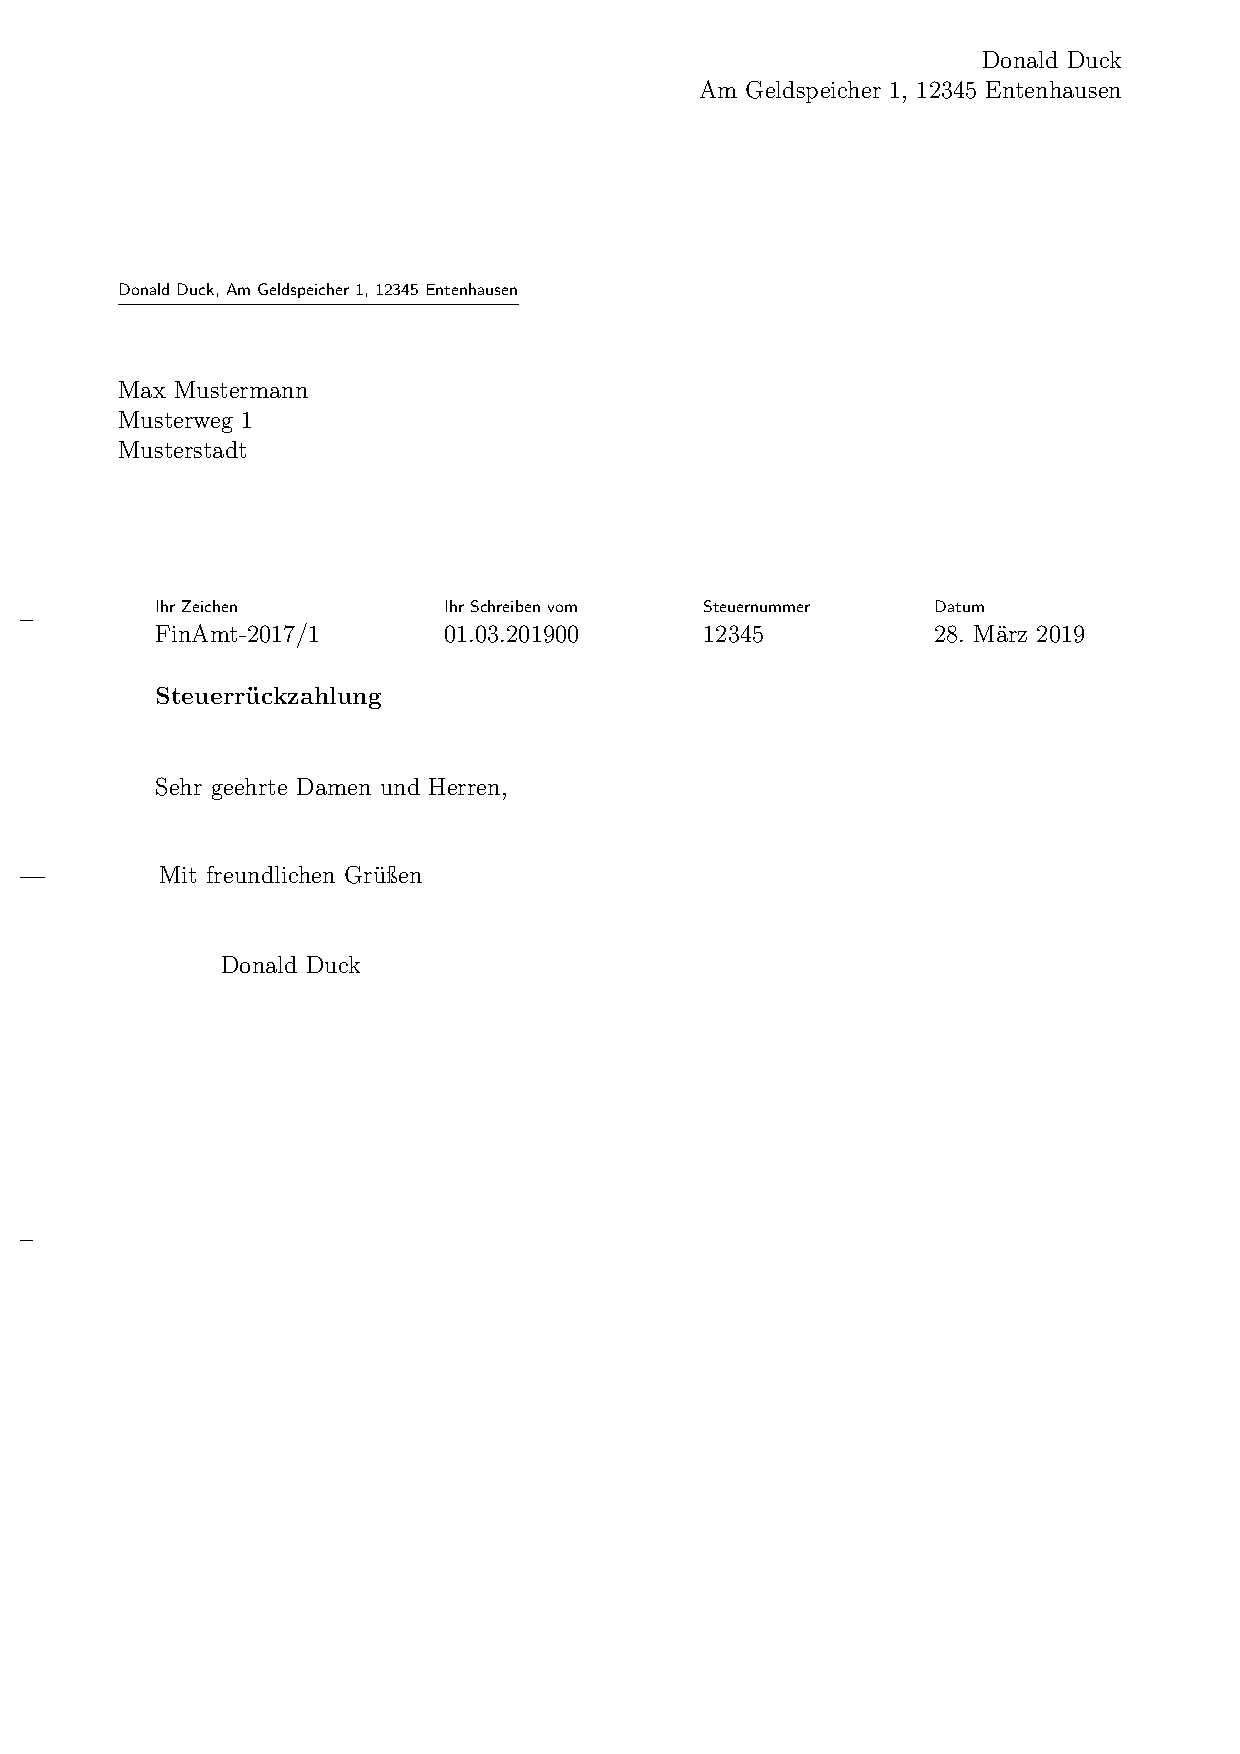
\includegraphics[trim=0cm 13.25cm 0cm 0.5cm, width=0.85\textwidth]{brief-08}}
\end{center}

\end{frame}


\begin{frame}
\frametitle{fromalign=off}

\vspace*{-0.75cm}\begin{center}
\fbox{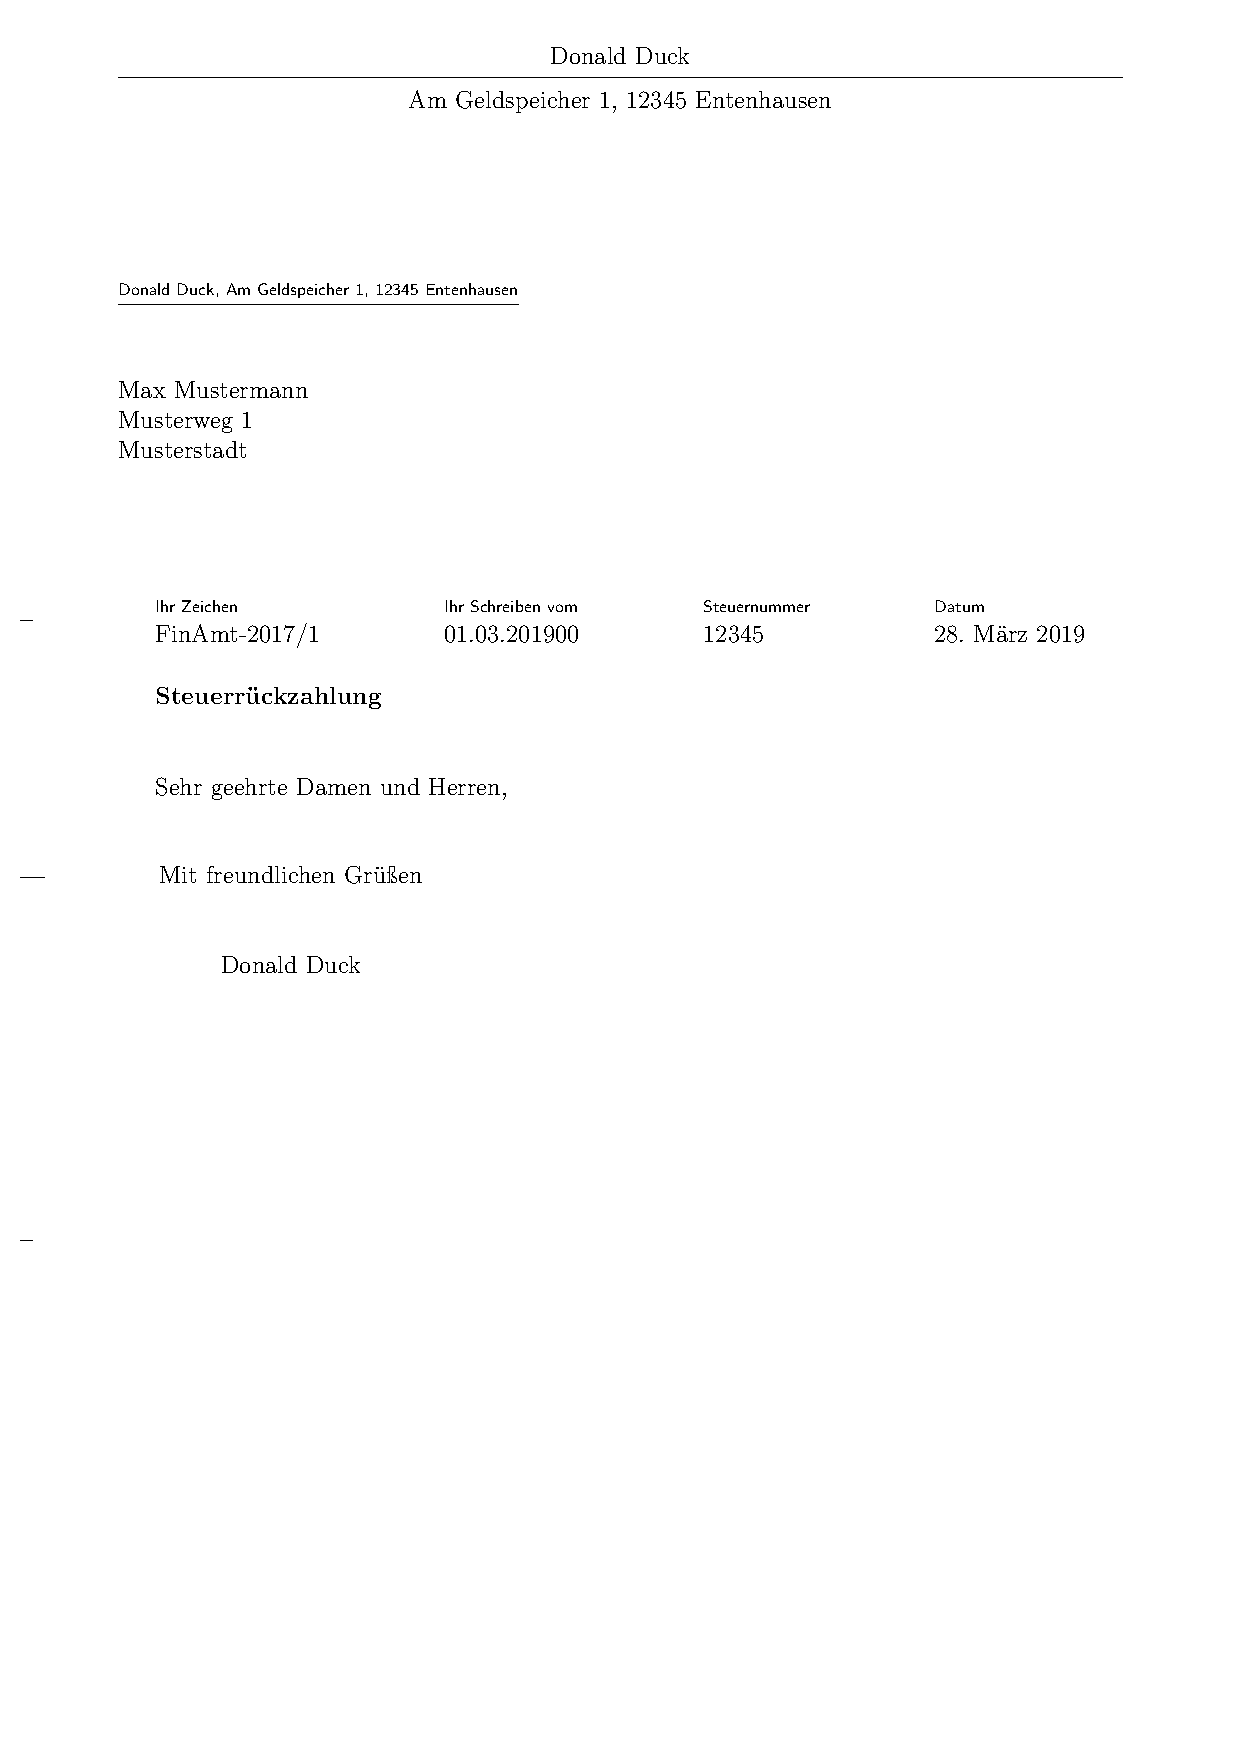
\includegraphics[trim=0cm 13.25cm 0cm 0.5cm, width=0.85\textwidth]{brief-09}}
\end{center}

\end{frame}

\begin{frame}
\frametitle{\texttt{\textbackslash usepackage\{sourcesanspro\}}}

\vspace*{-0.75cm}\begin{center}
\fbox{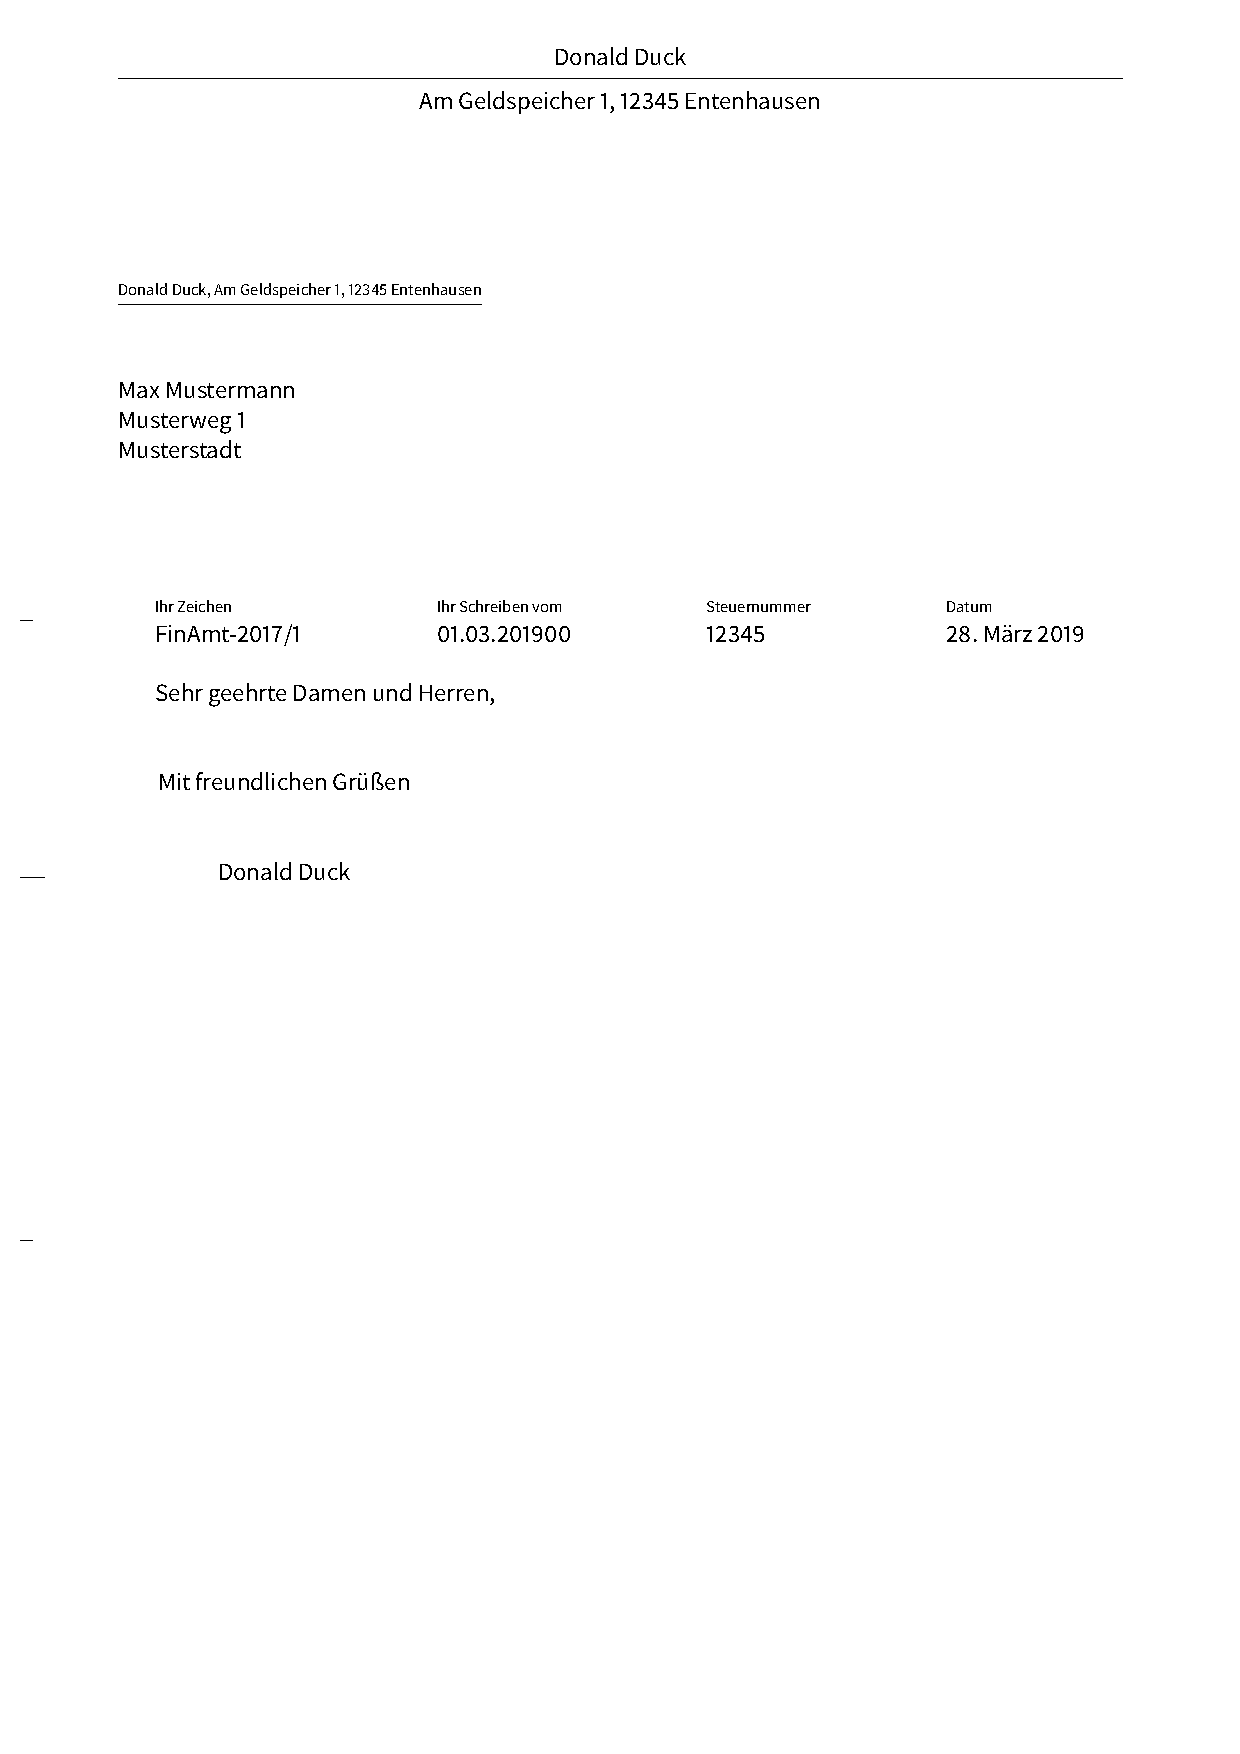
\includegraphics[trim=0cm 13.25cm 0cm 0.5cm, width=0.85\textwidth]{brief-10}}
\end{center}

\end{frame}

\begin{frame}
\frametitle{\texttt{\textbackslash usepackage\{tgchorus\}}\footnote{mit der \enquote{egreg}-Option}}

\vspace*{-0.75cm}\begin{center}
\fbox{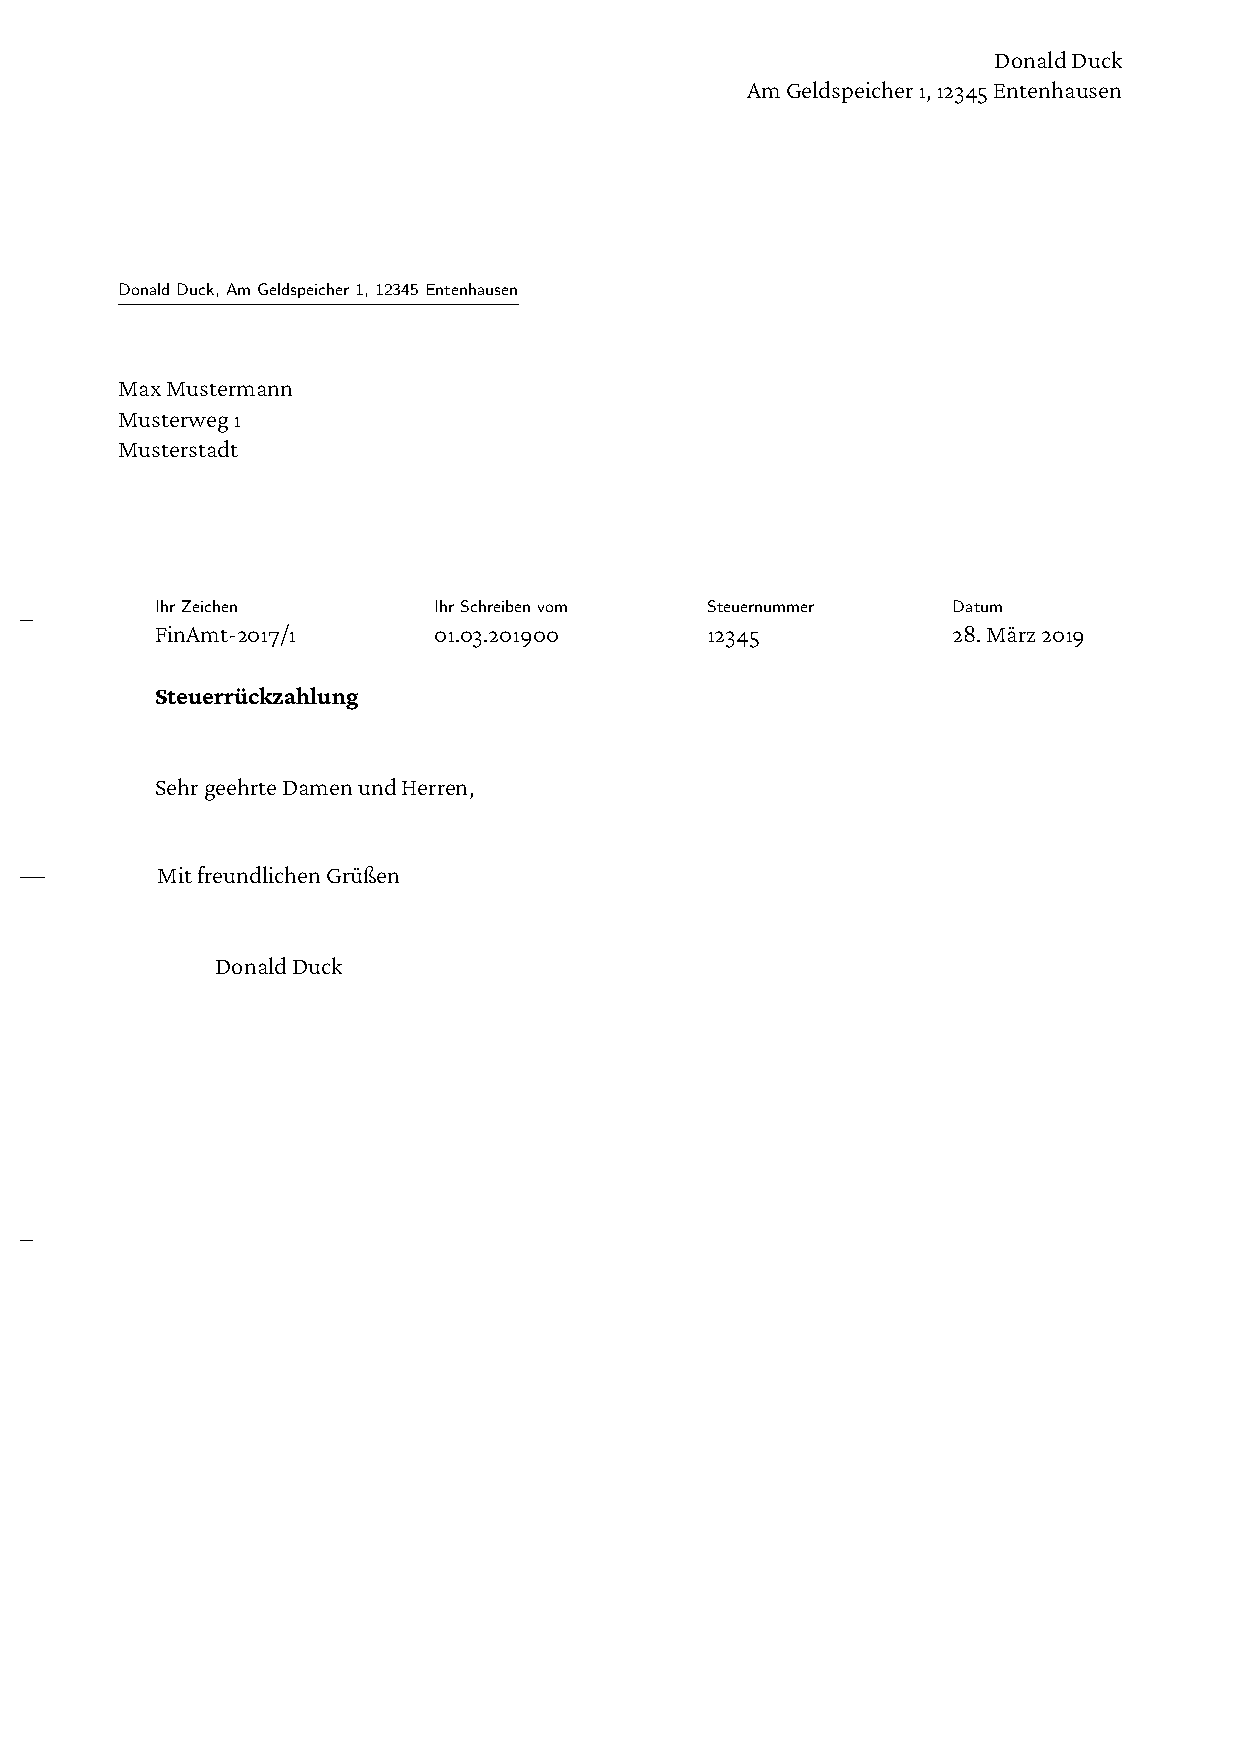
\includegraphics[trim=0cm 13.25cm 0cm 0.5cm, width=0.85\textwidth]{brief-11}}
\end{center}

\end{frame}


\begin{frame}
\frametitle{\texttt{\textbackslash usepackage[urw-garamond]\{mathdesign\}}\footnote{mit der \enquote{egreg}-Option}}

\vspace*{-0.75cm}\begin{center}
\fbox{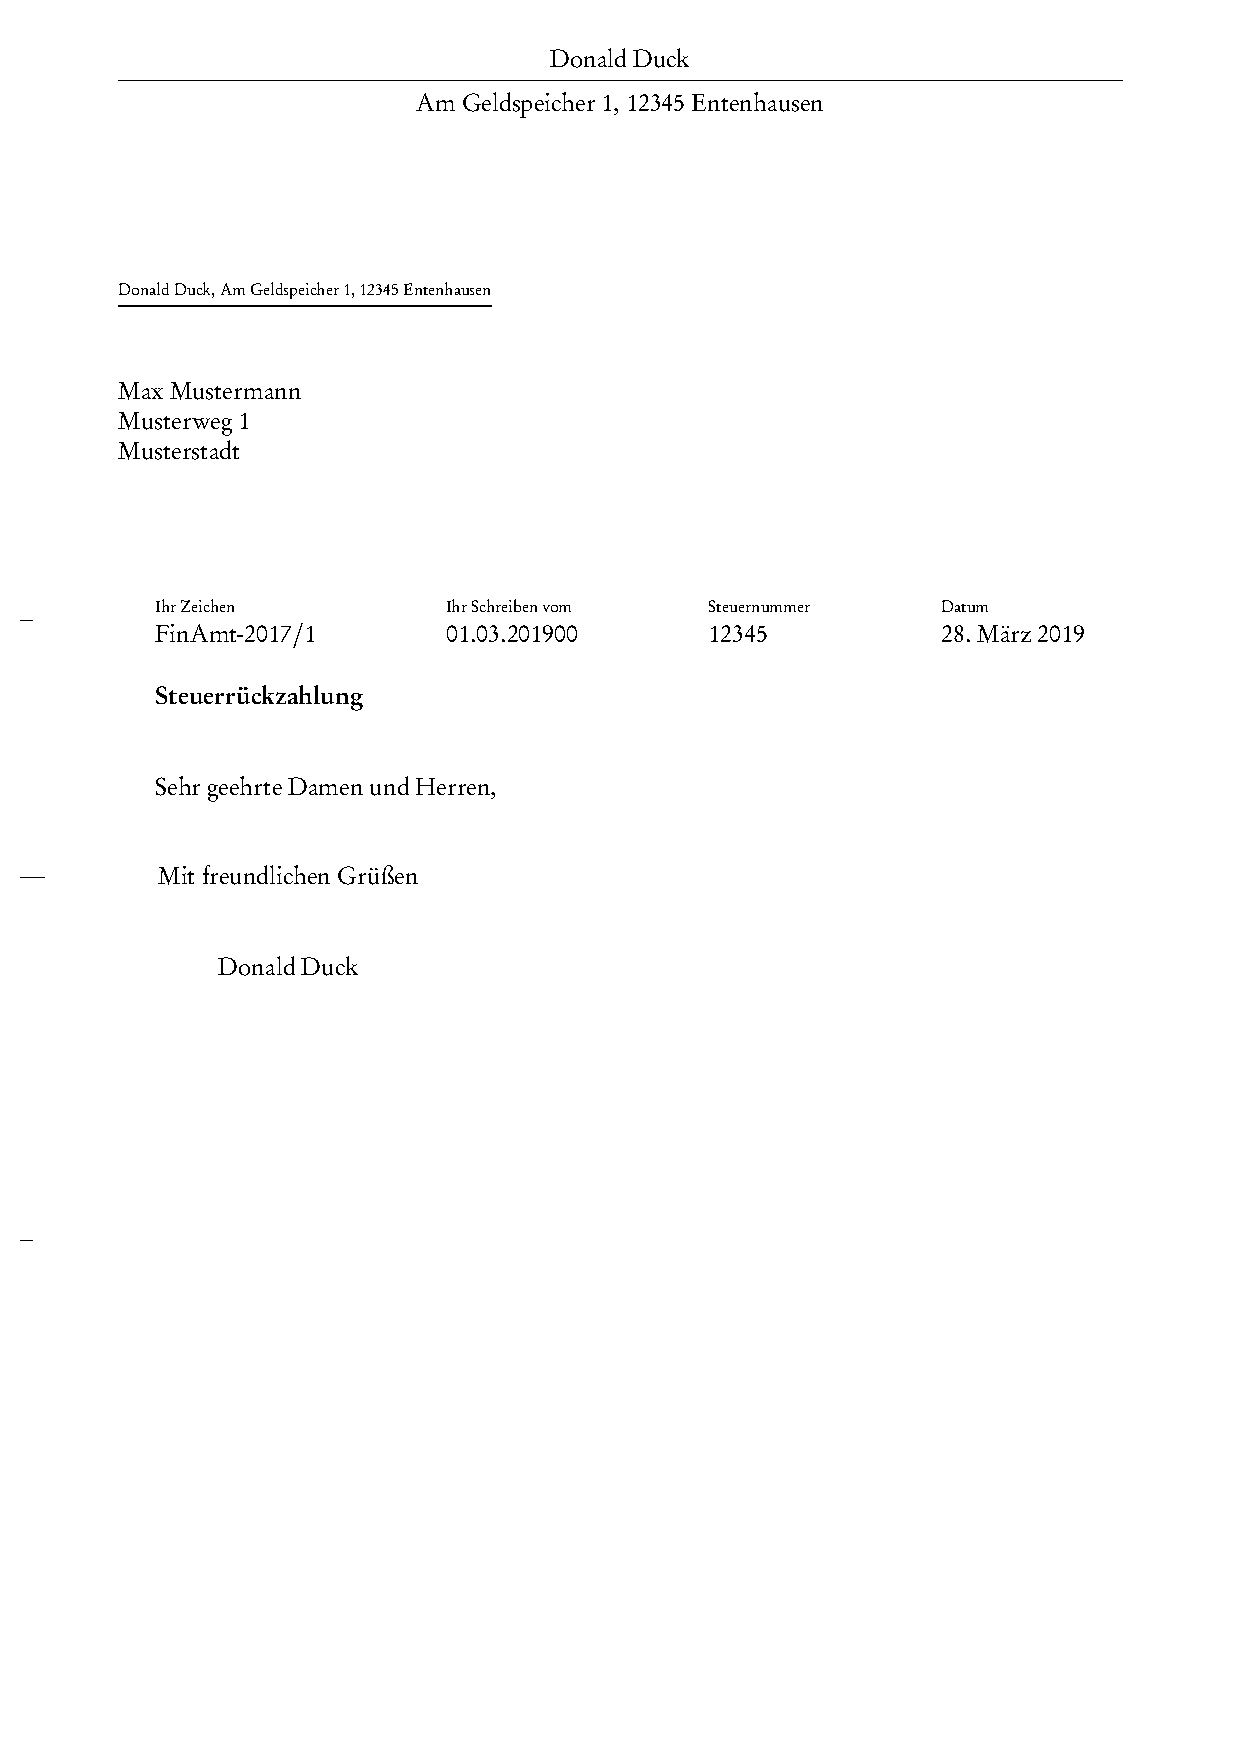
\includegraphics[trim=0cm 13.25cm 0cm 0.5cm, width=0.85\textwidth]{brief-12}}
\end{center}
\end{frame}

\begin{frame}
\frametitle{\texttt{\textbackslash usepackage[urw-garamond]\{mathdesign\}}\footnote{ohne \enquote{egreg}-Option}}

\vspace*{-0.75cm}\begin{center}
\fbox{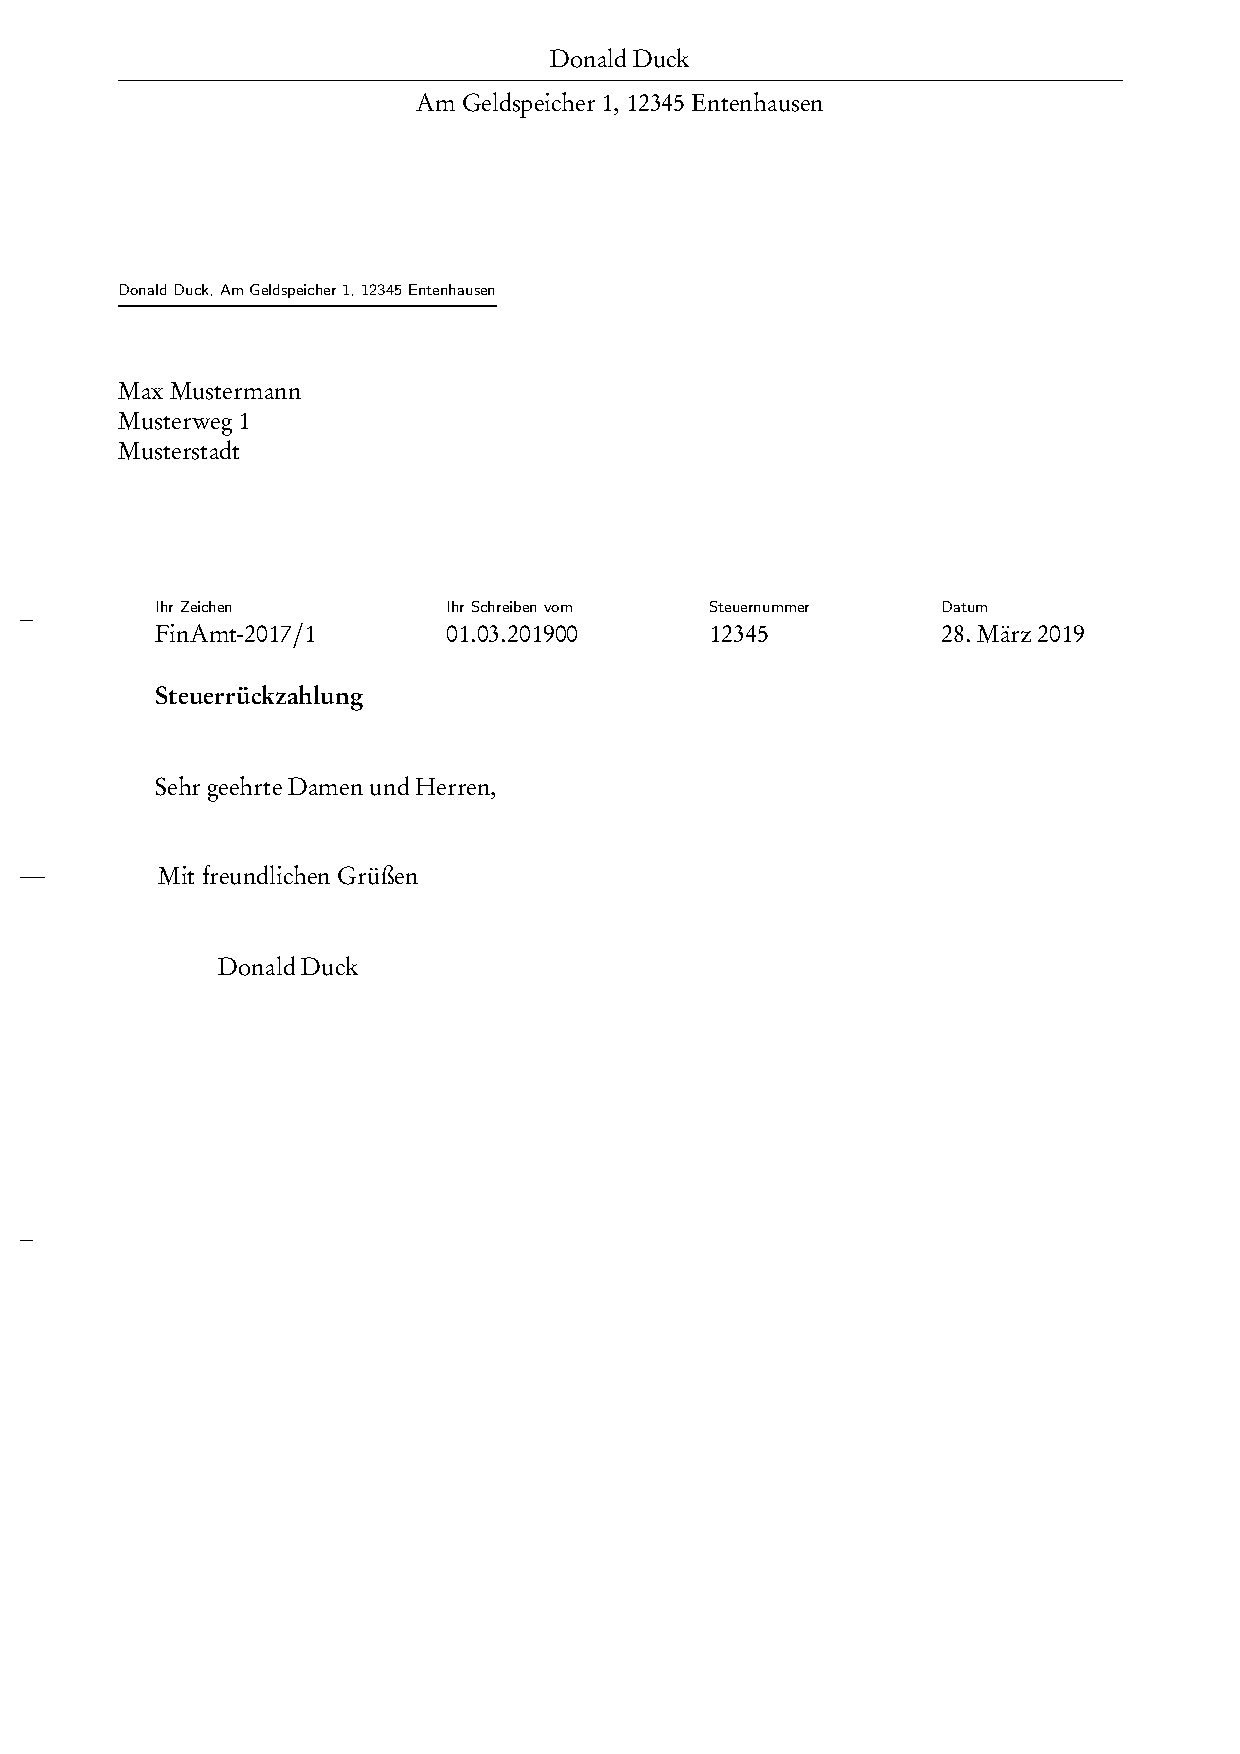
\includegraphics[trim=0cm 13.25cm 0cm 0.5cm, width=0.85\textwidth]{brief-13}}
\end{center}

\end{frame}


\begin{frame}[containsverbatim]
\frametitle{Auslagern von Absender-Informationen}

\begin{itemize}
\item Absenderinformationen und Design-Anweisungen können in \texttt{.lco} ausgelagert werden
\item sinnvoll für statische Informationen, nicht für Informationen, die sich in jedem Brief ändern.
\item (um Platz in Listings zu sparen, mache ich im folgenden genau dies)
\item einfacher Aufruf als Klassenoption:
\end{itemize}

\lstinputlisting[basicstyle=\ttfamily\footnotesize]{Donald.lco}


\end{frame}


\begin{frame}[containsverbatim]
\frametitle{firsthead/nexthead \& firstfoot/nextfoot}

\begin{itemize}
\item Kopf- und Fußzeile lassen sich individuell anpassen
\item \verb|\setkomavar{firsthead}{Inhalt}|
\item \verb|\setkomavar{firstfoot}{Inhalt}|
\item \verb|\setkomavar{nexthead}{Inhalt}|
\item \verb|\setkomavar{nextfoot}{Inhalt}|
\end{itemize}
\end{frame}

\begin{frame}[fragile]
\frametitle{Beispiel Bankverbindung in Fußzeile}

\begin{itemize}
	\item Nutzung der eingebauten Variablen \texttt{frombank}
	\item Benennen des Labels in \enquote{IBAN}
	\item Ausgabe von Label und Variablenwert in Fußnote auf erster Seite
\end{itemize}

\lstinputlisting[basicstyle=\ttfamily\footnotesize,firstline=7, lastline=10]{brief-14.tex}

\end{frame}

\begin{frame}[containsverbatim]
\frametitle{Beispiel Bankverbindung}

\begin{center}
\fbox{
\includegraphics[height=0.8\textheight]{brief-14}}
\end{center}

\end{frame}

\begin{frame}[containsverbatim]
\frametitle{Beispiel Bankverbindung}

\textbf{Ausgabe vergrößert}

\begin{center}
\fbox{
\includegraphics[width=1\textwidth]{Brief14_footer}}
\end{center}

\end{frame}

\begin{frame}[containsverbatim]
\frametitle{Beispiel Bankverbindung mit BIC}

\begin{itemize}
\item IBAN reicht eigentlich, BIC oft verlangt
\item Definition und Befüllung einer neuen Variablen \enquote{BIC}
\end{itemize}

\lstinputlisting[basicstyle=\ttfamily\footnotesize,firstline=7, lastline=14]{brief-15.tex}

\end{frame}

\begin{frame}
\frametitle{Komplexere Beispiele}

\begin{center}
\fbox{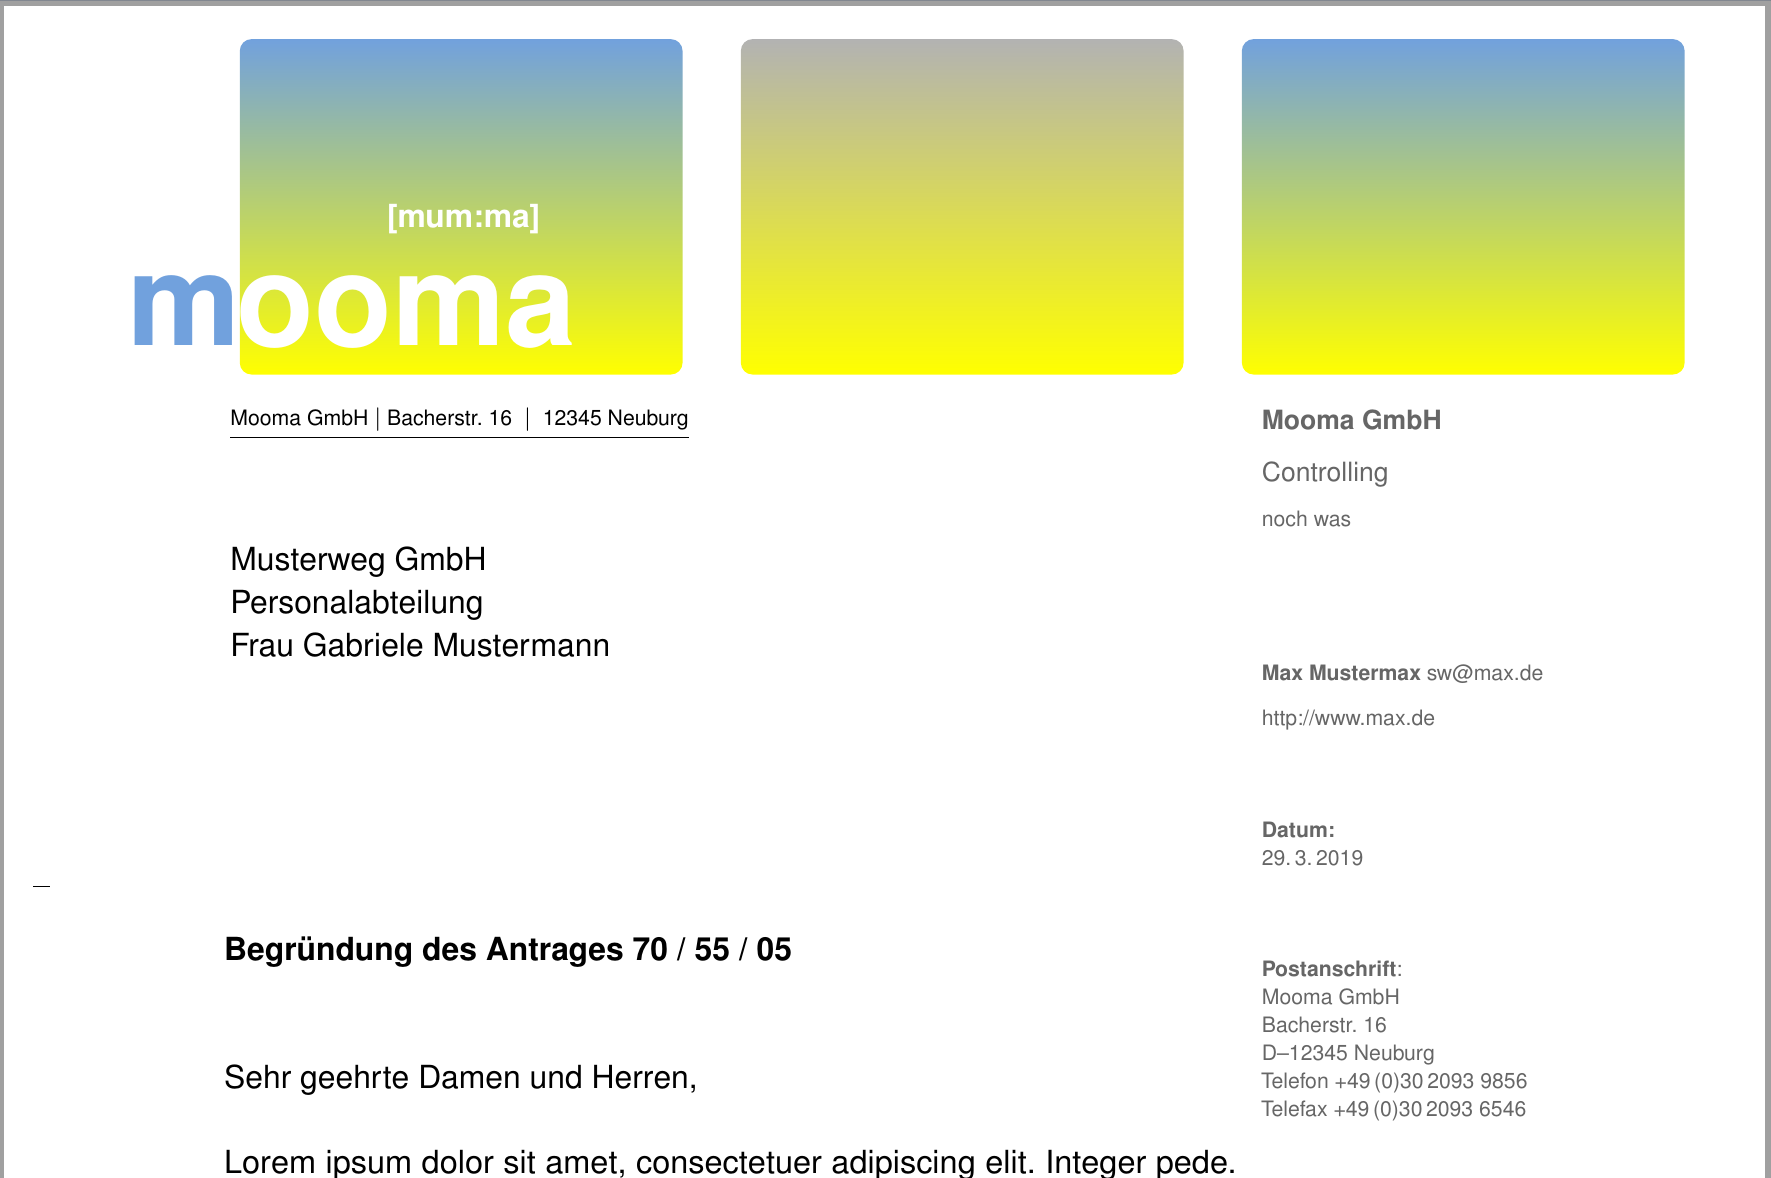
\includegraphics[width=1\textwidth]{mooma}}
\end{center}


\end{frame}



\end{document}